\section{MMO}\label{sec:mmo}

In this section, we introduce the MMO (\motivation, \means, \oportunity) schema. We contend that a malicious device, just like a human criminal, needs Motive, Means, and Opportunity to perpetuate its attack. Using this schema, we can better understand the DMA vulnerabilities of an OS, the viability of possible DMA attacks, and their prevention. 

For example, using MMO schema, we are able to lay out the necessary conditions for a successful privilege escalation attack (i.e., code injection). Specifically, a malicious device needs all three prerequisites:
\begin{enumerate}
    \item \motivation: A kernel buffer filled with malicious code (e.g., a valid ROP attack) -- a \mabaf.
    \item \means: The kernel virtual address (\kva) of a \mabaf. Given the device is using \iova, the attacker needs to obtain the relevant \kva{}, for example, by observing leaked pointers. 
    \item \oportunity: Write access to a known pointer, which can alter the CPU control flow. For example, write access to a data structure that holds a function callback pointer, at a known offset\footnote{The Linux kernel randomizes the layout of some data structures with \_\_randomize\_layout annotation \cite{rand_layout}.}.
\end{enumerate}

Another example is a full memory dump attack, which can be executed by merely having \oportunity. In this case, we are able to modify the kernel control flow in such a way as to cause it to dma\_map arbitrary kernel addresses at will. In order to achieve this, an attacker will need to modify a kernel pointer once before it is mapped and for a second time before send (i.e., TX) completion in order to avoid memory corruption (Section \ref{sec:linux_net}). 

To further emphasize the significance of the MMO attributes, we present a hypothetical scenario. Assume a NIC has write access to a page containing an RX packet (i.e., a received packet). Due to sub-page vulnerability and a random allocation coincidence, a structure with a callback pointer is inadvertently accessible with write permission. Also, the malicious device is able to create a valid \mabaf{} in the aforementioned page. It may seem that the device has a valid attack, whereas it actually lacks two essential prerequisites.

\begin{itemize}
    \item Missing \means: Without a valid \kva{} of the writable page, the device can not modify the callback function pointer to indicate the \mabaf.
    \item Missing \oportunity: Although a callback function pointer is available for modifications, the device has no way of knowing: 
    \begin{enumerate}
        \item[(a)] That a callback function pointer is available for sabotage.
        \item[(b)] The correct offset of the callback function pointer.
    \end{enumerate}
\end{itemize}

Under the hypothesized circumstance, and without additional information, a malicious device has practically no valid attack options. 
And while corrupting random kernel memory is still a possibility and may even cause a kernel panic \cite{MMT16}, it does not achieve the goal of privilege escalation.

\begin{figure}[t]
    \centering
    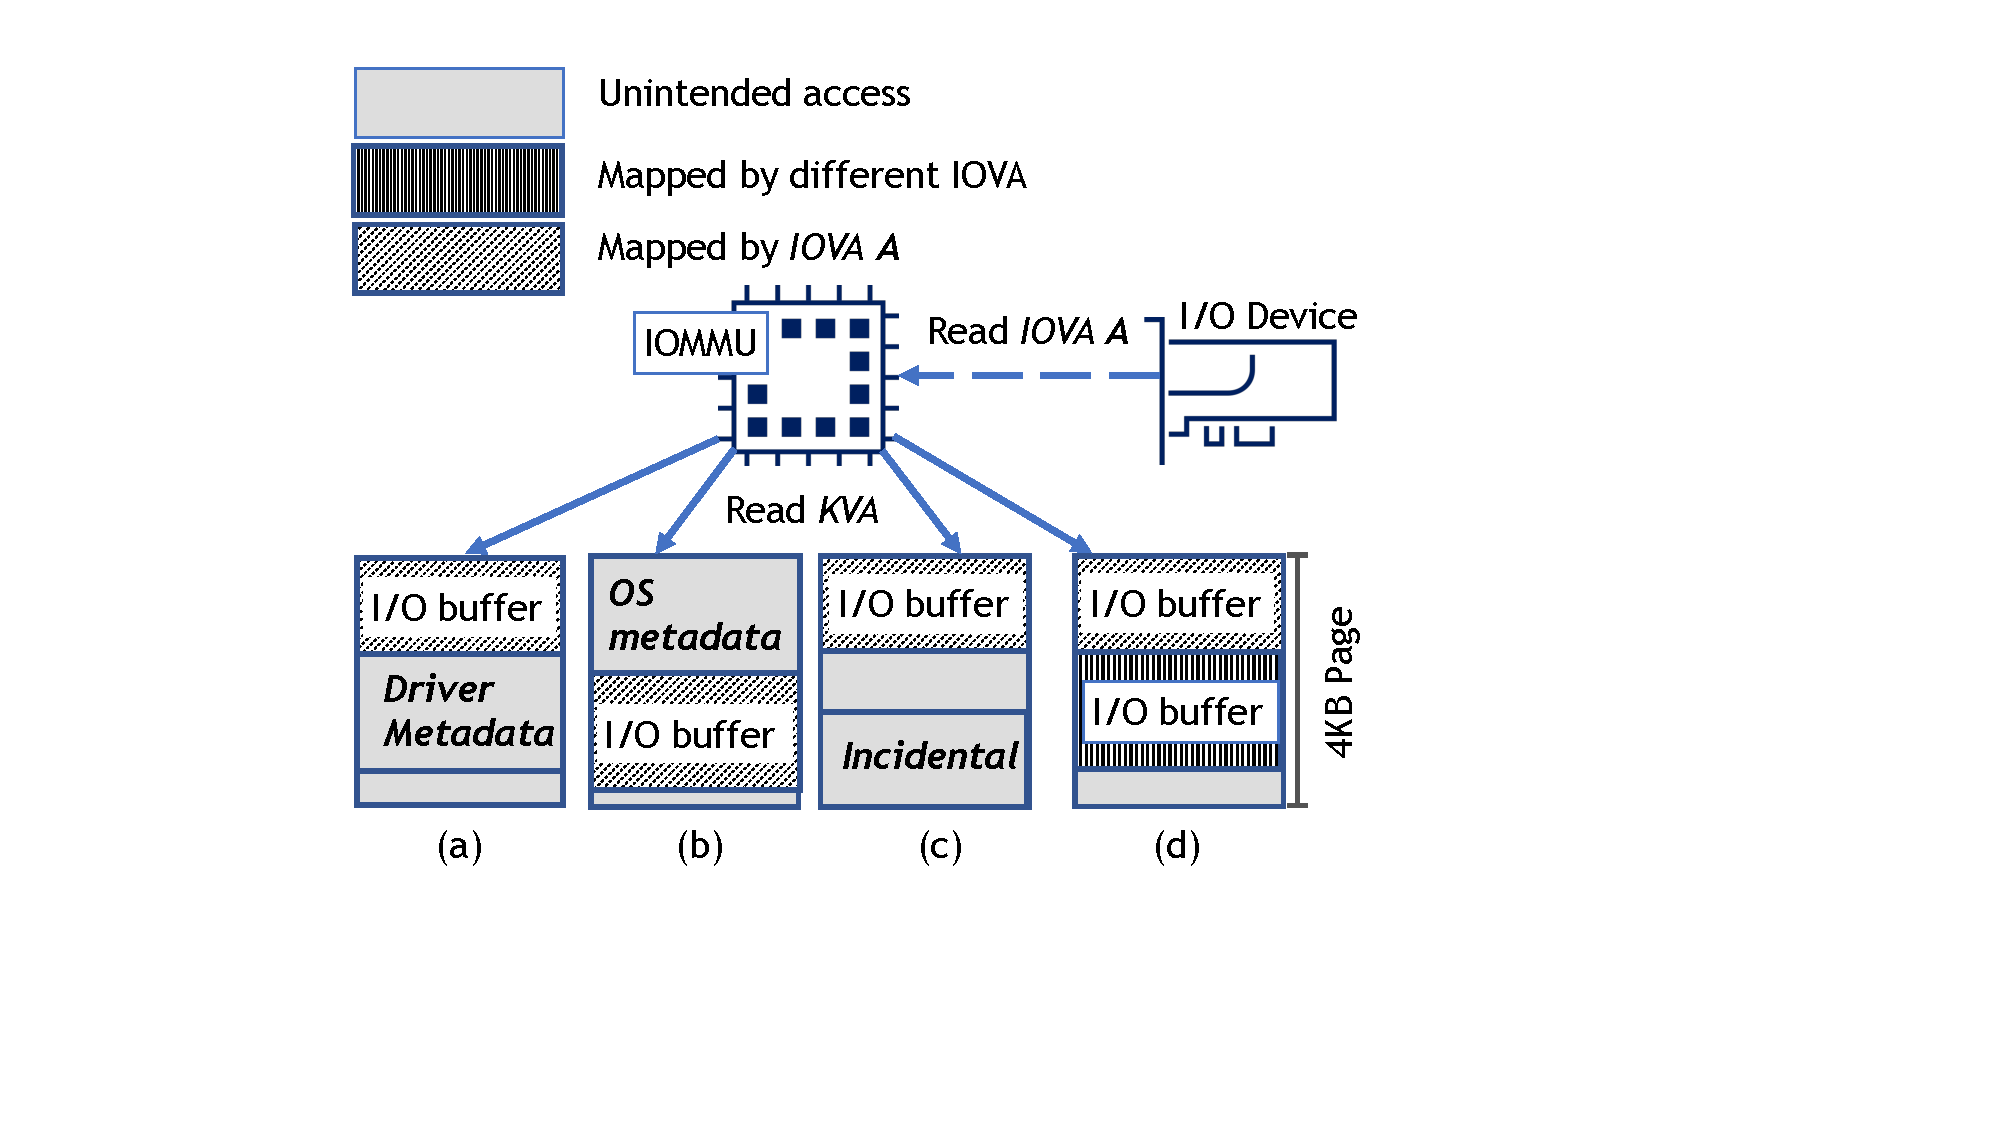
\includegraphics[width=1\columnwidth]{figs/subpage.pdf}
    \caption{Sub-page DMA vulnerabilities when the I/O buffer shares a page with other data: (a) I/O buffer metadata; (b) memory allocator’s
metadata; (c) randomly co-located sensitive buffers; (d) a page mapped by multiple \iova.}
    \label{fig:colocation}
\end{figure}

\subsection{Sub-Page Vulnerability}\label{sec:subpage}

We classify the different types of potentially co-located data, into four categories, as illustrated in Figure~\ref{fig:colocation}:

\begin{enumerate}
    \item[(a)] The I/O buffer is part of a bigger data structure. In some cases, this data structure may include function pointers, often caused by poor DMA hygiene by the driver. We demonstrate a full exploit in section \ref{sec:sbp2_attack}. An isolated driver fix is needed to solve such vulnerabilities.
    \item[(b)] The OS (e.g., memory allocator) rather than the driver saves metadata, such as free-lists, on the same page as the I/O buffer \cite{Cor07}. Manipulating these data structures may also compromise the system \cite{ak09}. Similarly to (a), sensitive metadata is shared. However, in this case, its an OS subsystem that is at fault rather than the device driver. We demonstrate attacks made possible by an OS subsystem in section \ref{sec:linux_net}.
    \item[(c)] The I/O buffer and a different, dynamically allocated memory buffer may coincidentally share a page. This common situation results in data leakage (e.g., kernel pointers).
    Currently, the Linux kernel uses the same memory allocation mechanism (e.g., kmalloc) for both I/O buffers and regular kernel buffers. Consequently, I/O buffers often share pages with other, potentially sensitive, kernel buffers. Since IOMMU works in page granularity, the respective I/O devices gain access to these kernel buffers as well. This is a subclass of (b), as an OS subsystem causes it, but the main difference is that the exposed data structures are leaked randomly.
     \item[(d)] The same page is mapped multiple times due to co-located device driver buffers resulting in multiple \iova{} to the same page. A seemingly benign case, made dangerous by the fact that unmapping one \iova{} is meaningless, security-wise. The device will retain access to the physical page as long as a single valid \iova{} exists. We discuss the implications of this scenario in section \ref{sec:linux_net}.
\end{enumerate}

\begin{figure*}[t]
    \centering
    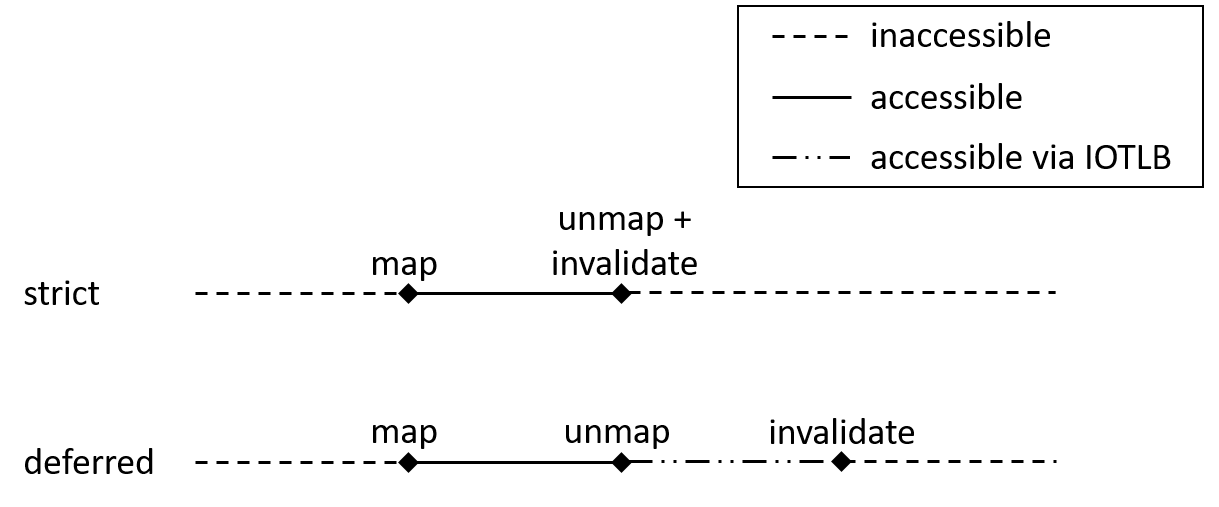
\includegraphics[width=1.3\columnwidth]{figs/deferred.png}
    \caption{Strict vs. deferred IOTLB invalidation. In \emph{deferred} mode, there is a time window where the data is accessible to the device, but the mapping no longer appears in the page table.}
    \label{fig:deferred}
\end{figure*}
\subsection{Static Analysis Tool}

Inspired by the MMO schema, we devise a static code analysis tool to classify device drivers by levels of risk. With well over a 1000 \texttt{dma\_map*} function calls, in the Linux Kernel alone, a manual process would be arduous.
Our static analysis tool flags drivers where \means{} or \oportunity{} are present. In the case of I/O devices \motivation{} is usually trivial as the device has legitimate write access and can freely write a poisoned ROP stack in any legitimate write accessible buffer. The tool looks for \texttt{dma\_map*} functions and traces back the call stack to identify if the mapped buffer is embedded inside a data structure (Fig. \ref{fig:colocation} (a)); additionally we look for hazardous functions (e.g., \texttt{build\_skb}), that create a data structure inside a mapped buffer (Fig. \ref{fig:colocation} (b)). The risk is classified according to the access permission, \motivation{}, implied by a READ permission, or \oportunity{} , implied by a WRITE/BIDIRECTIONAL permission. The case of multiple \iova{} (Fig. \ref{fig:colocation} (d)), is not a risk category by itself, rather a possible exploit. The tool flags use of functions (e.g., netdev\_alloc\_frag, napi\_alloc\_frag) that may result in this type of vulnerability.
Finally, the output of the tool presents structured and filtered findings conductive for more in-depth human expert analysis to determine if a viable attack is feasible. 

\noindent\textbf{Remark.} Option (c) falls under the category of random access attacks and as such, requires a more profound human expert dynamic analysis. As mentioned, this is out of the scope of this paper.


\subsection{Deferred Invalidation vulnerability} 

To limit the overhead of multiple memory accesses when translating \iova{} using the page tables, the IOMMU caches translations in an I/O translation lookaside buffer (IOTLB). 

The IOTLB is analogous to the MMU TLB. IOMMU does not maintain consistency between the IOTLB and the IOMMU page tables. As a result, the OS has to explicitly invalidate the IOTLB to maintain consistency when a translation entry is removed. Namely, to ensure that the IOTLB never holds stale entries, the OS must invalidate the IOTLB immediately after it removes memory mappings. 

Yet, this scheme, called the \emph{strict} mode in Linux, can degrade performance, as IOTLB invalidations can induce very high overhead \cite{MMT16,MSMT18,Peleg15}. In I/O intensive workloads, the number of required IOTLB invalidations can be extremely high, as IOMMU entries are unmapped following each I/O operation. Moreover, the overhead of each IOTLB invalidation can be as high as 2000 cycles \cite{ABYTS11}. This is considerably higher than a TLB invalidation, which takes roughly 100 cycles \cite{Han14}. 

To reduce this overhead, Linux defers TLB invalidations by default and instead performs periodic global TLB invalidations. While \emph{deferred} mode, improves I/O performance, it also breaks the stipulation, that after \texttt{dma\_unmap}, the physical page should no longer be accessible by the device. This \emph{deferred} time frame (Figure \ref{fig:deferred}), may be as high as 10 milliseconds \cite{MSMT18}.

The repercussions of \emph{deferred} mode are that a malicious device can take advantage of this time window, where it has access to memory pages, effectively, unbeknownst to the CPU. This opens up two distinct attack options:

\begin{enumerate}
    \item A device can alter data structures that the CPU has modified \emph{after} calling \texttt{dma\_unmap}.
    \iova{} mappings, as a rule, are short-lived as they should be used only for the duration of I/O, usually for a few microseconds. The additional milliseconds provide the attacker with a wide time-window sufficient to conduct his attack.
    \item The page can be freed, and then immediately reused by the OS. In fact, this is a common scenario, as Linux prefers to reuse \emph{hot} pages (i.e., recently used pages), as they are likely, to already reside in the CPU caches \cite{hotcold}. In turn, this opens up the kernel to an additional random access attack.
\end{enumerate}

We demonstrate in Section \ref{sec:linux_net}, how an adversary can take advantage of \emph{deferred} mode.

\subsection{Threat Model}

Our attacks are designed with the following assumptions:
\begin{enumerate}
    \item We assume the existence of a malicious DMA capable device attached to the system.
    \item The actual attack is performed solely by a DMA-capable malicious device.
    \item Any hardware aside from the specific malicious device is working as expected.
    \item Any ports intended for debugging (e.g., jtag), are not considered.
 \end{enumerate}

The most significant potential consequence of our attacks is privilege escalation, which allows attackers to execute arbitrary code with kernel privileges. Another potential consequence we consider is a full system memory dump; these are harder to thwart and even harder to detect.  
Lastly, a consequence of a possible failed attack is random memory corruption, resulting in a denial of service \cite{MMT16}, where the OS panics. Ideally, malformed devices should not be able to crash the entire system. 